%% http://www.cmake.org/Wiki/CMake/Tutorials/How_to_create_a_ProjectConfig.cmake_file

\documentclass[12pt,a4wide]{article}

\usepackage{color}
\usepackage{listings}
\lstset{basicstyle=\small\ttfamily,
  breaklines=true,
  showstringspaces=false,
  commentstyle=\color{green},
  keywordstyle=\bf\color{black},
  stringstyle=\color{red},
  language=make,
  morekeywords={mkdir,macro,endmacro,string,if,else,endif,
    include_directories, find_package, add_executable, target_link_libraries}
}

\renewcommand{\today}{January 6, 2015}
% Requires Python package Pygments
%\usepackage{minted}

\usepackage{hyperref}

\title{\Large Deploying libraries using
  CMake\\
\normalsize
or how to use find\_package}

\usepackage{tikz}
\usetikzlibrary{trees}

\makeatletter
\newcount\dirtree@lvl
\newcount\dirtree@plvl
\newcount\dirtree@clvl
\def\dirtree@growth{%
  \ifnum\tikznumberofcurrentchild=1\relax
  \global\advance\dirtree@plvl by 1
  \expandafter\xdef\csname dirtree@p@\the\dirtree@plvl\endcsname{\the\dirtree@lvl}
  \fi
  \global\advance\dirtree@lvl by 1\relax
  \dirtree@clvl=\dirtree@lvl
  \advance\dirtree@clvl by -\csname dirtree@p@\the\dirtree@plvl\endcsname
  \pgf@xa=.5cm\relax
  \pgf@ya=-.5cm\relax
  \pgf@ya=\dirtree@clvl\pgf@ya
  \pgftransformshift{\pgfqpoint{\the\pgf@xa}{\the\pgf@ya}}%
  \ifnum\tikznumberofcurrentchild=\tikznumberofchildren
  \global\advance\dirtree@plvl by -1
  \fi
}

\tikzset{
  dirtree/.style={
    scale=.7,
    font={\scriptsize\ttfamily},
    growth function=\dirtree@growth,
    every node/.style={anchor=north},
    every child node/.style={anchor=west},
    edge from parent path={(\tikzparentnode\tikzparentanchor) |- (\tikzchildnode\tikzchildanchor)}
  }
}
\makeatother


\begin{document}
\maketitle

\section{Introduction}
Native CMake projects that are intended to be used by other projects
(e.g. libraries) must provide information like include-directories,
libraries, required compile-flags and locations of executables. A
structured way of doing this is by using CMake's
\lstinline{find_package} command in config-mode. In this document, an
example of systematically generating project configuration files,
which can be used by \lstinline{find_package} is given. The example is
an elaboration of what can be found at
\href{http://www.cmake.org/Wiki/CMake/Tutorials/How\_to\_create\_a\_ProjectConfig.cmake\_file}{http://www.cmake.org/Wiki/}. This
guide is not a full introduction to CMake or \lstinline{find_package},
but rather a demonstration of some experienced I have made by using
the KitWare's recommended way of deploying libraries using CMake.

\section{The command \lstinline{find_package}}
The command \lstinline{find_package} is often used in module-mode,
where the find-modules are files like \lstinline{FindXXX.cmake}. Many
find-modules provide limited or no support for versioning and they do
not support propagating configurations like required compiler flags,
secondary dependencies etc. If you do not consider deployment, stuff
like required compiler flags etc are usually done by inheritance, but
in a large hierarchy, it can be quite difficult to figure out where a
given flag is set and you often have to run CMake in verbose. Writing
\lstinline{ProjectConfig.cmake} is a way of avoid this trouble.

A small example of how to use a generated
\lstinline{ProjectConfig.cmake} is given below:
\begin{lstlisting}[frame=single,title=Using a library foo from a package FooBar]
find_package(FooBar 0.6 CONFIG)
include_directories("${FOOBAR_INCLUDE_DIRS}")
add_executable(main client.c)
target_link_libraries(main foo)
\end{lstlisting}
There is no need to use the CONFIG option. If no find-module
\lstinline{FindFooBar.cmake} is found and the MODULE option is not
given the command proceeds to config-mode. In this example a location
of the include-directories is exported using the variable \lstinline{FOOBAR_INCLUDE_DIRS}.

Benefits from using config-mode rather than module-mode, when using \lstinline{find_package}:
\begin{itemize}
 \item No need to maintain FindXXX.cmake files
 \item Systematic way for enforcing compiler flags or any other configuration across projects
 \item  Many find-modules provide limited or no support for versioning
 \item Versioning is handled in a generic way - the version number only
   resides in automatically generated files (which can extract version
   from a versioning system)
 \item Possiblity for deploying libraries
 \item Easy to enforce a directory structure, which is compatible with
   both local development and installed libraries
\end{itemize}

\section{Using libraries}
The command \lstinline{find_package} searches for dependencies using the directory structure in the
following order \lstinline{/usr/local/include},
\lstinline{/usr/include}, \lstinline{/usr/target/include},
\lstinline{/usr/include}. On Windows, this is handled using the
registry. An important point is that a developers path is searched
before local install locations or system-wide install
locations. On Windows, the search order is:
\begin{enumerate}
  \item Developers debug version (if debugging)
  \item Developers release version
  \item Installed version
\end{enumerate}
For all dependencies, the version requirements must be met, i.e
versioning have precedence over location.

In the example above, the following can be added to support dynamic
libraries on Windows

\begin{lstlisting}[frame=single,title=Using a dynamic library foo from a package FooBar]
find_package(FooBar 0.6 CONFIG)

set(USE_SHARED_LIBS ON)

# Static or dynamic
if ("${FOOBAR_RUNTIME_DIR}" STREQUAL "")
  set(USE_SHARED_LIBS OFF)
endif()

include_directories("${FOOBAR_INCLUDE_DIRS}")
add_executable(main client.c)
target_link_libraries(main foo)

if (USE_SHARED_LIBS)
  # Check if the library is installed or under development
  string( FIND ${FOOBAR_RUNTIME_DIR_RELEASE} "bin" APOSITION )
  if (${APOSITION} EQUAL -1)
    # Library is under development
    add_custom_command(TARGET main POST_BUILD
        COMMAND ${CMAKE_COMMAND} -E copy_if_different
            "${FOOBAR_RUNTIME_DIR}/$<CONFIGURATION:main>/${FOOBAR_RUNTIME_LIBRARIES}"
    "$<TARGET_FILE_DIR:main>")
  else()
    # Library is installed
    add_custom_command(TARGET main POST_BUILD
        COMMAND ${CMAKE_COMMAND} -E copy_if_different
            "${FOOBAR_RUNTIME_DIR_RELEASE}/${FOOBAR_RUNTIME_LIBRARIES}"
    "$<TARGET_FILE_DIR:main>")
  endif()
endif()
\end{lstlisting}

\section{Simple example}
In this example a single library foo is deployed together with an
application bar. The deployment and configuration is handled using
autogenerated project configuration files.

In this example the following aspects are handled
\begin{itemize}
  \item Propagation of version information (built to install)
  \item Version verification
  \item Install and development usage
  \item Directory naming
  \item Movement of binaries (Windows)
  \item RPath binary headers (Unix)
\end{itemize}

\subsection{Source tree}
The source directory structure is as follows:
\begin{figure}[htbp]
\begin{center}
\begin{minipage}[c]{.9\columnwidth }
  \centering
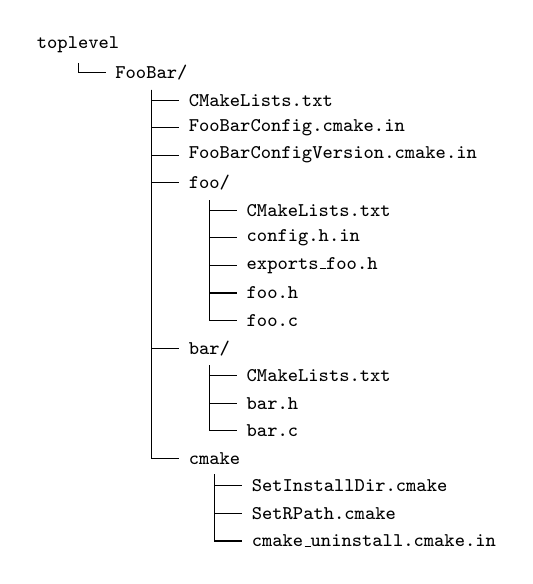
\begin{tikzpicture}[dirtree]
\node{toplevel}
  child { node  {FooBar/}
    child { node {CMakeLists.txt}}
    child { node {FooBarConfig.cmake.in}}
    child { node {FooBarConfigVersion.cmake.in}}
    child { node  {foo/}
      child { node {CMakeLists.txt}}
      child { node {config.h.in}}
      child { node {exports\_foo.h}}
      child { node {foo.h}}
      child { node {foo.c}}
    }
    child { node {bar/}
      child { node {CMakeLists.txt}}
      child { node {bar.h}}
      child { node {bar.c}}
    }
    child { node {cmake}
      child { node {SetInstallDir.cmake}}
      child { node {SetRPath.cmake}}
      child { node {cmake\_uninstall.cmake.in}}
    }
  };
\end{tikzpicture}
\end{minipage}
\end{center}
\caption{Source directory structure for a package {\ttfamily FooBar}
  containing a library {\ttfamily foo} and an executable {\ttfamily bar}.}
\label{fig:foo_directory}
\end{figure}

The content of the \lstinline{FooBar/cmake} directory is macros, which
can be used for all projects - i.e. not project specific
\paragraph{\ttfamily FooBarConfig.cmake.in} Input to a project configuration file. It
  contains both static and dynamic content. The dynamic content is
  referring to variables declared in \lstinline{FooBar/CMakeList.txt},
  \lstinline{FOOBAR_INCLUDE_DIRS} is generated to reflect the actual
  location of the API header files.

\paragraph{\ttfamily FooBarConfigVersion.cmake.in} Input to version
  information, this way very well refer to variables initialized
  during checking out a tagged version of your source.
\paragraph{\ttfamily foo/config.h.in} Inputs, which are used during
  compilation, e.g. a version string or whether a system header is
  available or not.
\paragraph{\ttfamily foo/exports\_foo.h} Windows export functionality for
  shared libraries, we could name is \lstinline{exports.h}, if headers
  are deployed per library.
\paragraph{\ttfamily cmake/SetInstallDir.cmake} Rules about how the built
  and install tree look like.
\paragraph{\ttfamily cmake/SetRPath.cmake} Decision on how to use \lstinline{RPath},
  \lstinline{RUNPATH} and \lstinline{LD_LIBRARY_PATH}. This is
  relevant only on NIX platforms
\paragraph{\ttfamily cmake\_uninstall.cmake.in} Uninstall target for
Windows. On Unix, you can simply use {\ttfamily xargs rm < install\_manifest.txt}

\section{Built tree}
The built tree follows the rules on the given platform, e.g. on
Windows using Visual Studio, the output is placed in
\lstinline{BUILD_DIR/x64/Release} for a 64-bit built tree in the
release configuration. The only important note is that during
compilation the registry is updated, such that wherever you compile
your libraries, they can always be found by other projects using
\lstinline{find_package}. There is no need for decisions on naming or
locations of libraries during development.

\section{Install tree}
You can use any library by simply compiling them and
\lstinline{find_package} will search and find the given libraries. If
desired, a library or package can be deployed into an installation
tree. In this example, the installation tree is separating libraries,
binaries and include files, while maintaining all relative paths used
for inclusion. Further, all exported variables are adjusted to
facilitate development using an installed library - like shipping an
SDK. Installing the FooBar in \lstinline{toplevel}, results in the following:
\begin{figure}[htbp]
\begin{center}
\begin{minipage}[c]{.9\columnwidth }
  \centering
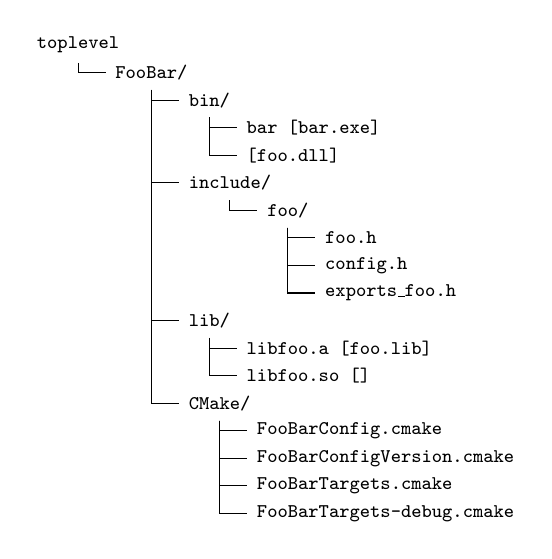
\begin{tikzpicture}[dirtree]
\node{toplevel}
  child { node  {FooBar/}
    child { node  {bin/}
      child { node {bar [bar.exe]}}
      child { node {[foo.dll]}}
    }
    child { node {include/}
      child { node {foo/}
        child { node {foo.h}}
        child { node {config.h}}
        child { node {exports\_foo.h}}
      }
    }
    child { node {lib/}
      child { node {libfoo.a [foo.lib]}}
      child { node {libfoo.so []}}
    }
    child { node {CMake/}
      child { node {FooBarConfig.cmake}}
      child { node {FooBarConfigVersion.cmake}}
      child { node {FooBarTargets.cmake}}
      child { node {FooBarTargets-debug.cmake}}
    }
  };
\end{tikzpicture}
\end{minipage}
\end{center}
\caption{Deployed development directory structure for a package {\ttfamily FooBar}
  containing a library \lstinline{foo} and an executable \lstinline{bar}.}
\label{fig:foo_directory}
\end{figure}

Some advantages include
\begin{itemize}
\item The library names are expressed in the include
hierarchy, i.e. you can use the following  
\begin{lstlisting}[language=c]
#include <foo/foo.h>
\end{lstlisting}
That is for all interface headers for all libraries you see where they
belong.
\item The top-level is now the package name {\ttfamily FooBar}, but
  this can be changed to say {\ttfamily SharedComponents}
\item Uninstall/install can easily work in a shared install tree and only
  remove or update the right components
\end{itemize}

\section{Macros}
The example is rather complicated and can be simplified a lot using
macros. As a simple example, the following:
\begin{lstlisting}
if (BUILD_SHARED_LIBS)
  set(FOOBAR_DYNAMIC_LINKING TRUE)
else()
  set(FOOBAR_DYNAMIC_LINKING FALSE)
endif()
\end{lstlisting}
can be replaced with \lstinline{setup_build("FooBar")} using this macro
\begin{lstlisting}
macro(setup_build _name)
  string(TOUPPER "${_name}" _upper_name)
  if (BUILD_SHARED_LIBS)
    set("${_upper_name}_DYNAMIC_LINKING" TRUE)
  else()
    set("${_upper_name}_DYNAMIC_LINKING" FALSE)
  endif()
endmacro()
\end{lstlisting}



\end{document}


%% Local variables:
%% TeX-master: "find_package.tex"
%% End:

% Local IspellDict: english
% Local IspellPersDict: ~/.aspell.en.pws
